\beginsong{Gregor}[txt={aus der Jungenschaft, niedergeschrieben von Eberhard Köbel und Günther Wolff, 1934}, mel={nach ukrainischem Volkslied}, bo={166}, pfii={104}, pfiii={65}, kssiv={40}, siru={87}, index={Gehe nicht, oh Gregor}]

\beginverse
\endverse

\centering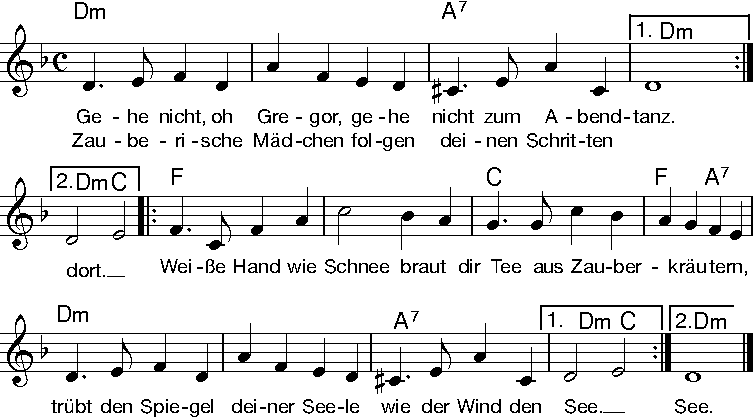
\includegraphics[width=1\textwidth]{Noten/Lied048.pdf}	

\beginverse
\[Dm]Dort ist auch die eine mit den \[A7]schwarzen Augen\[Dm]brauen.
Glaube mir, oh Gregor, das ist \[A7]eine Zaube\[Dm]rin.
\lrep \[C] \[F]Ihre schmale Hand braut dir \[C]Tee aus Zauber\[F]kräu\[A7]tern,
\[Dm]legt sich über deine Seele \[A7]wie der Herbst auf's \[Dm]Land.\rrep
\endverse

\beginverse
^Sonntag früh beim Glockenläuten ^grub sie aus das ^Kraut,
schnitt es Montag, alle Sünden ^hexte sie hi^nein,
\lrep ^ ^holt' es Dienstag vor, braute ^Zaubertrank aus den ^Kräu^tern,
^Mittwoch Nacht beim Reigentanze ^gab sie ihn Gre^gor.\rrep
\endverse

\beginverse
^Und am Tag darauf am Tage ^war Grischenko ^tot.
Freitag kam voll Leid und Klage ^und beim Abend^rot
\lrep ^ ^trug man ihn zur Ruh' an der ^Grenze an der ^Stra^ße.
^Viele fromme Leute kamen, ^sahen traurig ^zu.\rrep
\endverse

\beginverse
^Viele Knaben, viele Burschen ^klagten um Gre^gor.
Böse Hexe, Zauberhexe, ^schwarze Zauber^frau,
\lrep ^ ^deine Augenbrauen werden ^keinen mehr be^tö^ren,
^nie mehr wird ein zweiter Gregor ^deinen Künsten ^trau'n. \rrep
\endverse


\endsong

\beginscripture{}
Es handelt sich in dem Lied wahrscheinlich lediglich um ein Mädchen, das den geliebten Zigeuner Gregor vergiftet, weil es auf andere Frauen eifersüchtig ist.
\endscripture
